\documentclass[12pt]{article}
\usepackage[utf8]{inputenc}
\usepackage[T1]{fontenc}
\usepackage[left=2cm,right=2cm,top=2cm,bottom=2cm]{geometry}
\usepackage[french]{babel}
\usepackage{graphicx}
\usepackage{url}
\usepackage{hyperref}
\hypersetup{
    colorlinks,
    citecolor=black,
    filecolor=black,
    linkcolor=black,
    urlcolor=black
}
\bibliographystyle{alpha}


\begin{document}
	\begin{titlepage}
		
\includegraphics[scale=0.2]{logo_bordeaux.png}\\
		\centering
		{\LARGE \bfseries Université de Bordeaux}\\ [2cm]
		\textsc{\Large Master 1 Informatique}\\ [0,3cm]
		\textsc{\Large 2016/2017}\\ [1,5cm]

		\textsc{\Large Projet de programmation}\\ [1.5cm]


		\rule{16cm}{1mm}\\ [0,7cm]
		{ \huge \bfseries Visualisation de trajets de vélos en libre service} \\[0,5cm]
		{ \huge \bfseries Analyse des besoins}\\ [0,7cm]
		\rule{16cm}{1mm}\\ [1cm]

		{\Large Chargé de TD Boris MANSENCAL }\\ [0,3cm]
		{\Large Client Romain GIOT }\\ [1cm]

		{\Large Damien Bielawski }\\ [0,3cm]
		{\Large Sébastien Bielawski }\\[0,3cm]
		{\Large Alaric Braillon }\\ [0,3cm]
		{\Large Alassane Diop }\\ [2cm]
		\Large\today

	\end{titlepage}

	\tableofcontents \newpage

	\section{Introduction}
		Cette section a pour but de décrire et donner un aperçu sur le contenu de ce document d'analyse des besoins. Il présente aussi les recherches et ce qui a déjà été fait sur ce sujet.

		\subsection{Contexte}
			Le projet consiste en la réalisation d’un logiciel de visualisation de trajets d'un système de vélos en libre service. 
			Il est réalisé par quatre étudiants de première année de master informatique, dans le cadre d'une UE de projet de programmation.

		\subsection{Objectifs}
			Ce logiciel doit permettre la visualisation des trajets des systèmes de vélos en libre service. En utilisant les données mise à disposition par les villes et par des données récupérables sur le web, on peut récupérer les informations sur les trajets des utilisateurs dans une ville donnée. Ainsi, grâce à des filtres, on peut choisir quelle information on veut visualiser.\\
			Le logiciel est destiné aux personnes souhaitant analyser les trajets d'un système de vélos en libre service, grâce à des données libres. Il peut permettre l'analyse statistique des trajets, comme connaître le temps moyen d'un trajet des utilisateurs par exemple.

		\subsection{Définitions, acronymes}
			Il se peut que vous rencontriez des termes ou acronymes pour la première fois, cette section devrait vous aidez à les comprendre.
			\begin{itemize}
				\item[$\bullet$] BSS : bike sharing system, système de vélos en libre service
				\item[$\bullet$] CSV : Comma Separated Value, c'est un format de fichier
				\item[$\bullet$] JSON : format de fichier
				\item[$\bullet$] Qt : Est un framework très populaire pour le développement d'interfaces graphiques
				\item[$\bullet$] Doxygene : Outil permettant de générer de la documentation, en html, en latex ou XML par exemple.
			\end{itemize}

		\subsection{Description de l'existant}
			Une application a déjà été développée par des chercheurs. Il s’agit d’une application web qui a l’inconvénient d’être assez lente dès lors qu’il y a beaucoup de donnée à traiter. Les liens vers les deux vidéos montrent qu'il s'agit d'une application web ouverte avec Google Chrome. On peut aussi voir d'après l'url, qu'il s'agit d'une démonstration en local (localhost:8080). Nous supposons que les performances ne doivent pas être optimales avec ce type de technologie pour le web. Cependant nous ne savons pas combien de données ont été utilisées pour la démonstration.\\*\\*
			Aperçu de ce qui existe.\\*
			\url{https://drive.google.com/file/d/0B3aeg8yMfRj0MWFmUHZ6ZlR4MzA/view}\\*
			\url{https://drive.google.com/file/d/0B3aeg8yMfRj0R3VKQjdtX1htUUU/view}
		
		\subsection{Réferences}
			\begin{itemize}
				\item L'article \cite{Oli16} introduit clairement les problèmes rencontrés des systèmes de vélos en libre service. Notamment des problèmes d'équilibrage, de consommation de carburant pour les véhicules faisant la navette pour rééquilibrer les stations de vélos. On peut y puiser une grande source d'informations pour réaliser notre interface graphique. Ce sera le document sur lequel nous nous reposerons le plus.

				\item L'article \cite{Ali14} explique comment détecter les stations les plus connectées. Il donne un aperçu sur  l'utilisation des filtres (date, lieu, heure...).

				\item \cite{BC16} est un article sur les systèmes de partage de vélos. Il parle de l'application FunFEM qui permet de visualiser des données afin de juger de l'efficacité de ces systèmes.

				\item \cite{BSM17} est une application en ligne, qui permet de visualiser en temps réel des statistiques sur des bornes disponible dans une ville sélectionnée.  Elle indique également le nombre de vélos disponibles dans le monde en temps réel.

				\item L'article \cite{BW} de Ben Wellington, nous donne un bel aperçu sur la manière dont l'analyse statistique des données sur les utilisateurs du système de vélos en libre service peut être utilisée. Il montre comment les sociétés qui mettent à disposition les vélos dans la ville de New York pourraient augmenter leurs revenus grâce à une analyse des trajets des utilisateurs.

				\item \cite{JL} Recherches réalalisées sur la manière d'optimiser l'équilibrage des stations de vélos en libre service. Un des problèmes avec les stations de vélos est la gestion de l'équilibrage du nombre de  vélos dans chaque station. Il explique comment prédire à l'aide de données un épuisement de vélos dans certaines stations. Ainsi, à l'aide d'analyses d'une multitude de données sur la météo ou l'âge des utilisateurs par exemple, il est possible de d'optimiser la répartition des vélos et de faire des prédictions.

				\item Vidéo postée par Oliveira G \cite{state_station}, qui présente l'interface graphique de l'application web. Les différentes visualisations sont principalement portées sur l'analyse statistique des stations dans une ville donnée.

				\item Vidéo postée par Oliveira G \cite{trips}, qui présente cette fois une interface portée sur l'analyse des trajets. On peut séléctionner différents types de filtres.

			\end{itemize}
	\newpage
			

	\section{Expression des besoins}
		Cette section fournit une description detaillée des besoins de l'utilisateur aussi bien fonctionnels que non-fonctionnels.

		\begin{figure}[!ht]
		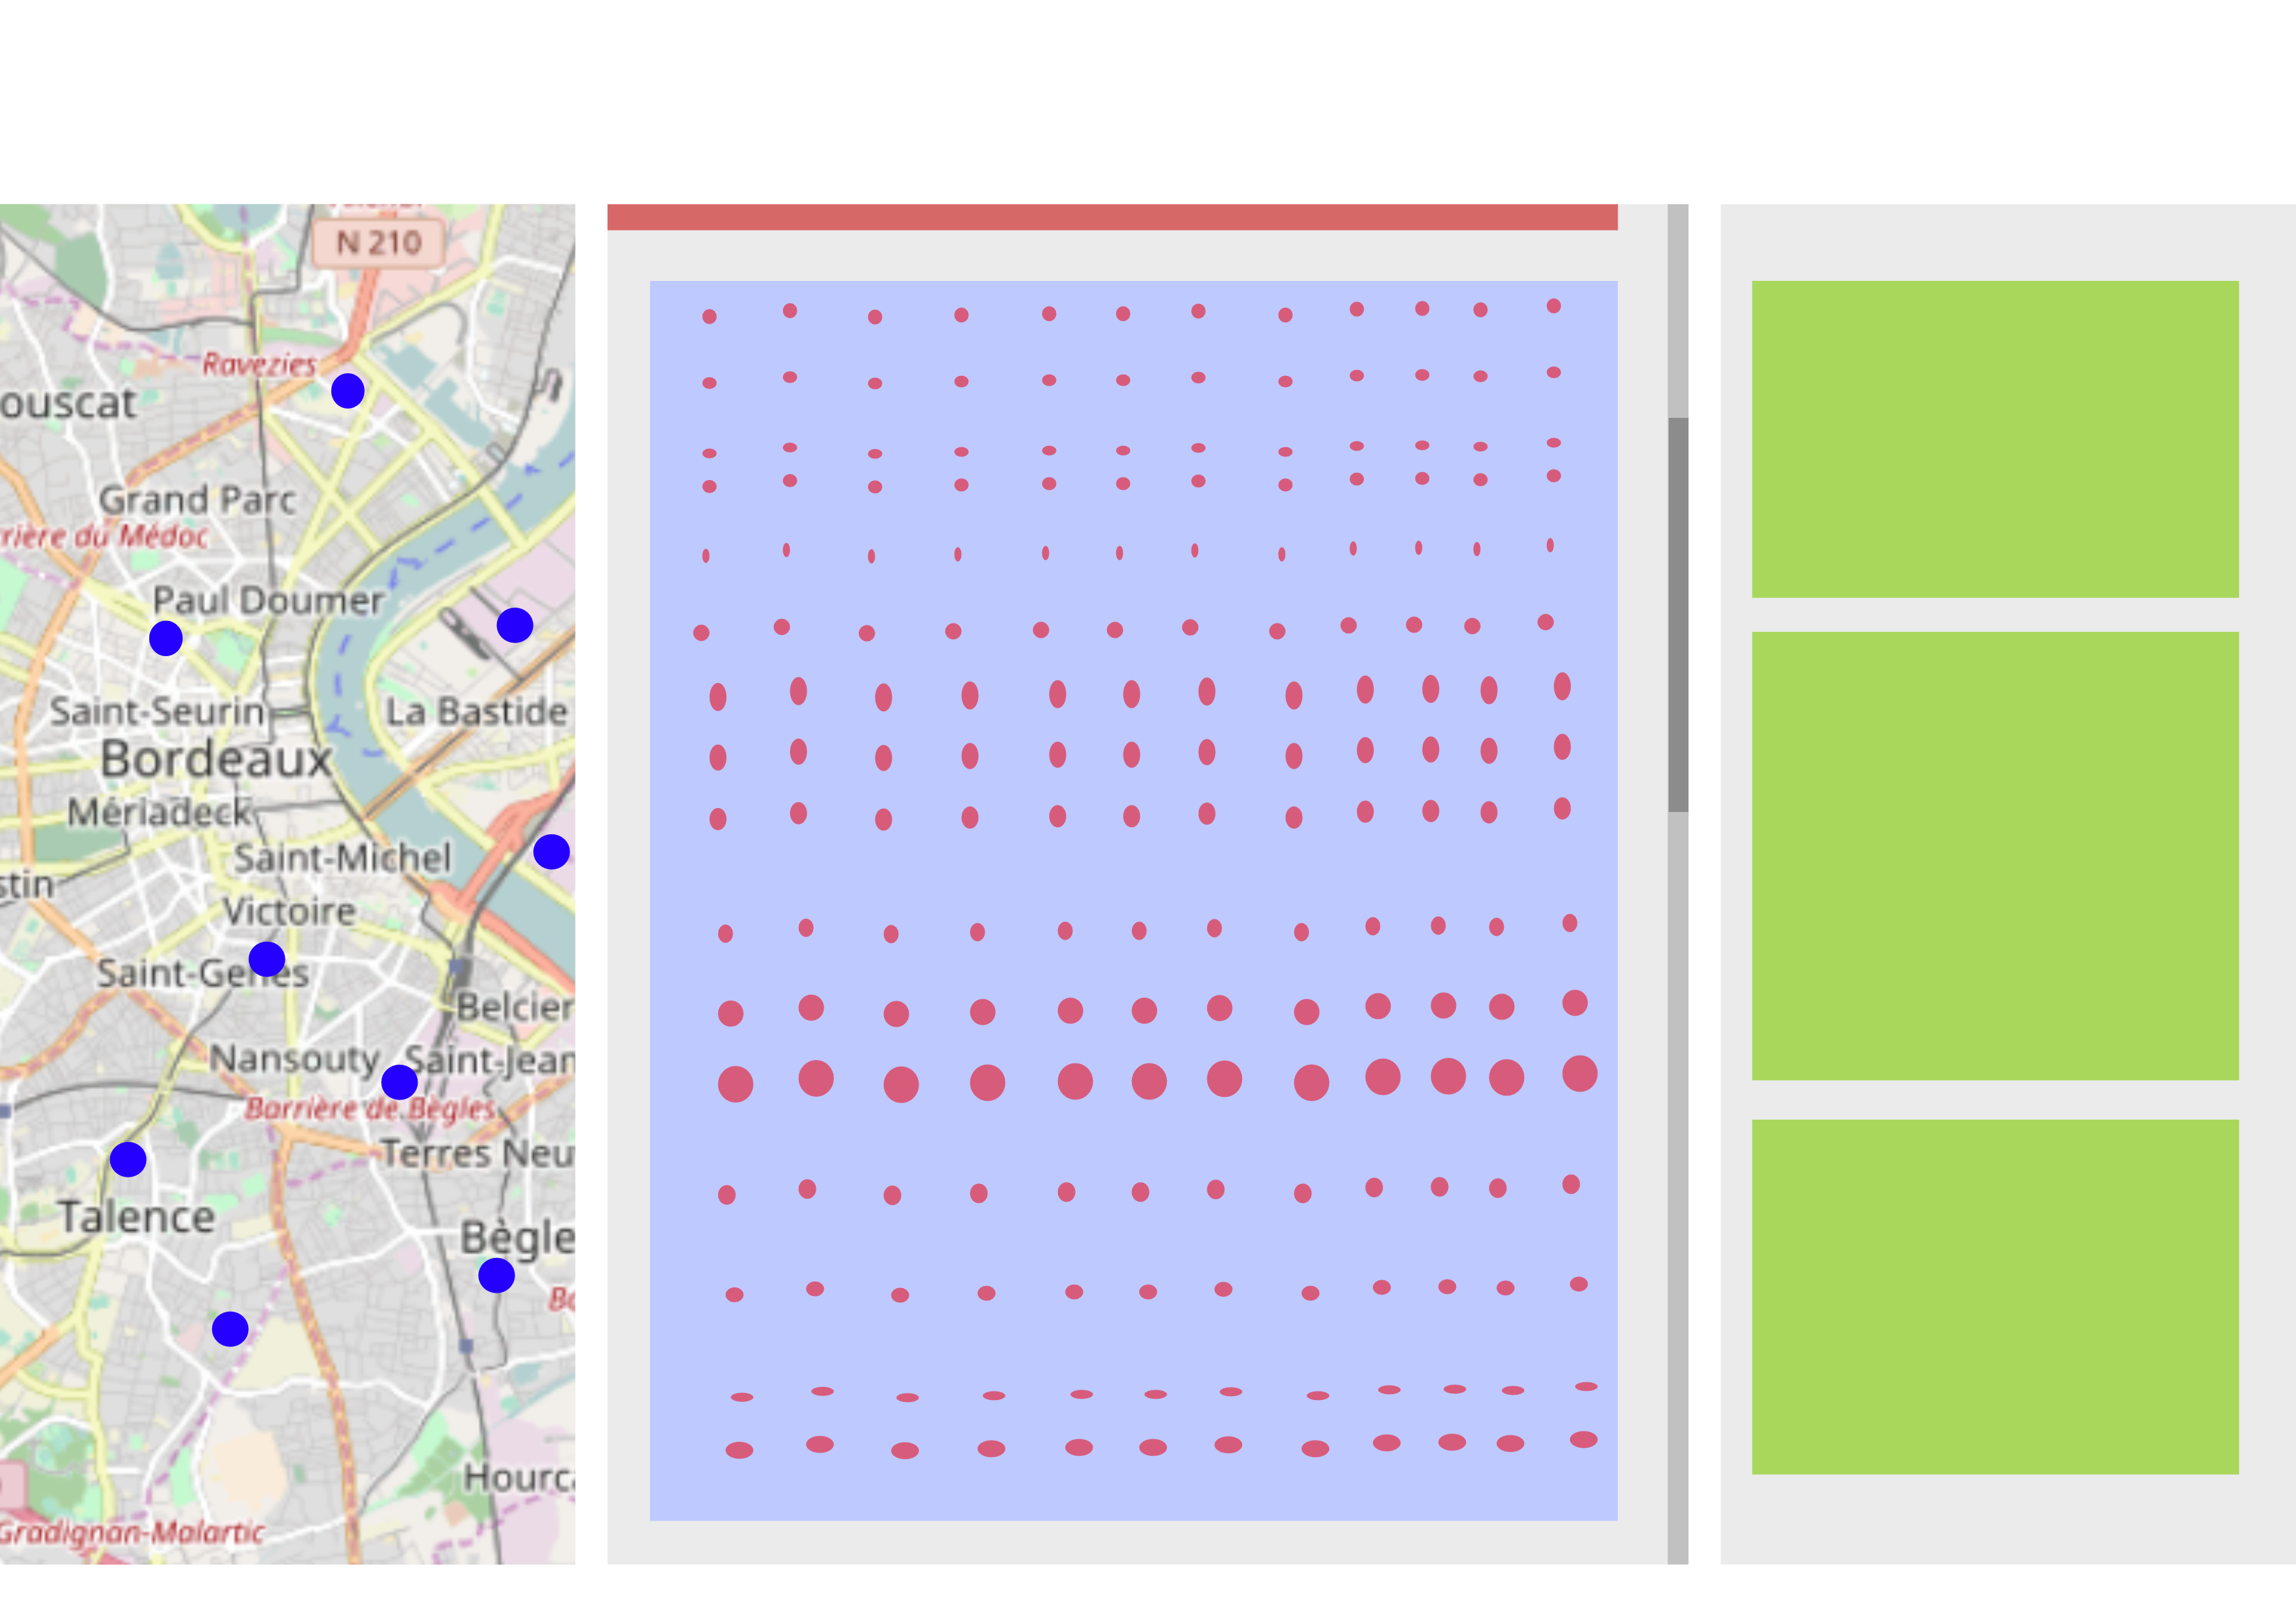
\includegraphics[scale=.5]{maquette.png}
		\caption{Maquette de l'interface graphique.}
		\medskip
		Elle se décompose principalement en trois parties.\par

		La fenêtre à gauche illustre la map de la ville avec les stations selectionnées.
		C'est elle qui va dessiner les trajets filtrés et selectionnés par l'utilisateur.\par

		La fenêtre au centre s'appelle la matrice de chronologie des trajets ("trips timeline matrix").
		C'est un tableau à double-entrées qui représente les trajets par stations dans le temps.
		Dans chaque cellule, il y a de petites étoiles rouges-bleues pour répresenter les trajets d'une station.
		Une ligne symbolise donc l'activité d'une station, elle est illustrée au cours du temps à intervalle régulier.\par

		Enfin, la fenêtre de droite va contenir les contrôles (tirettes, menu déroulants, cases à cocher...) pour modifier les paramètres de filtrage.
		\end{figure}

		\begin{figure}[!ht]
		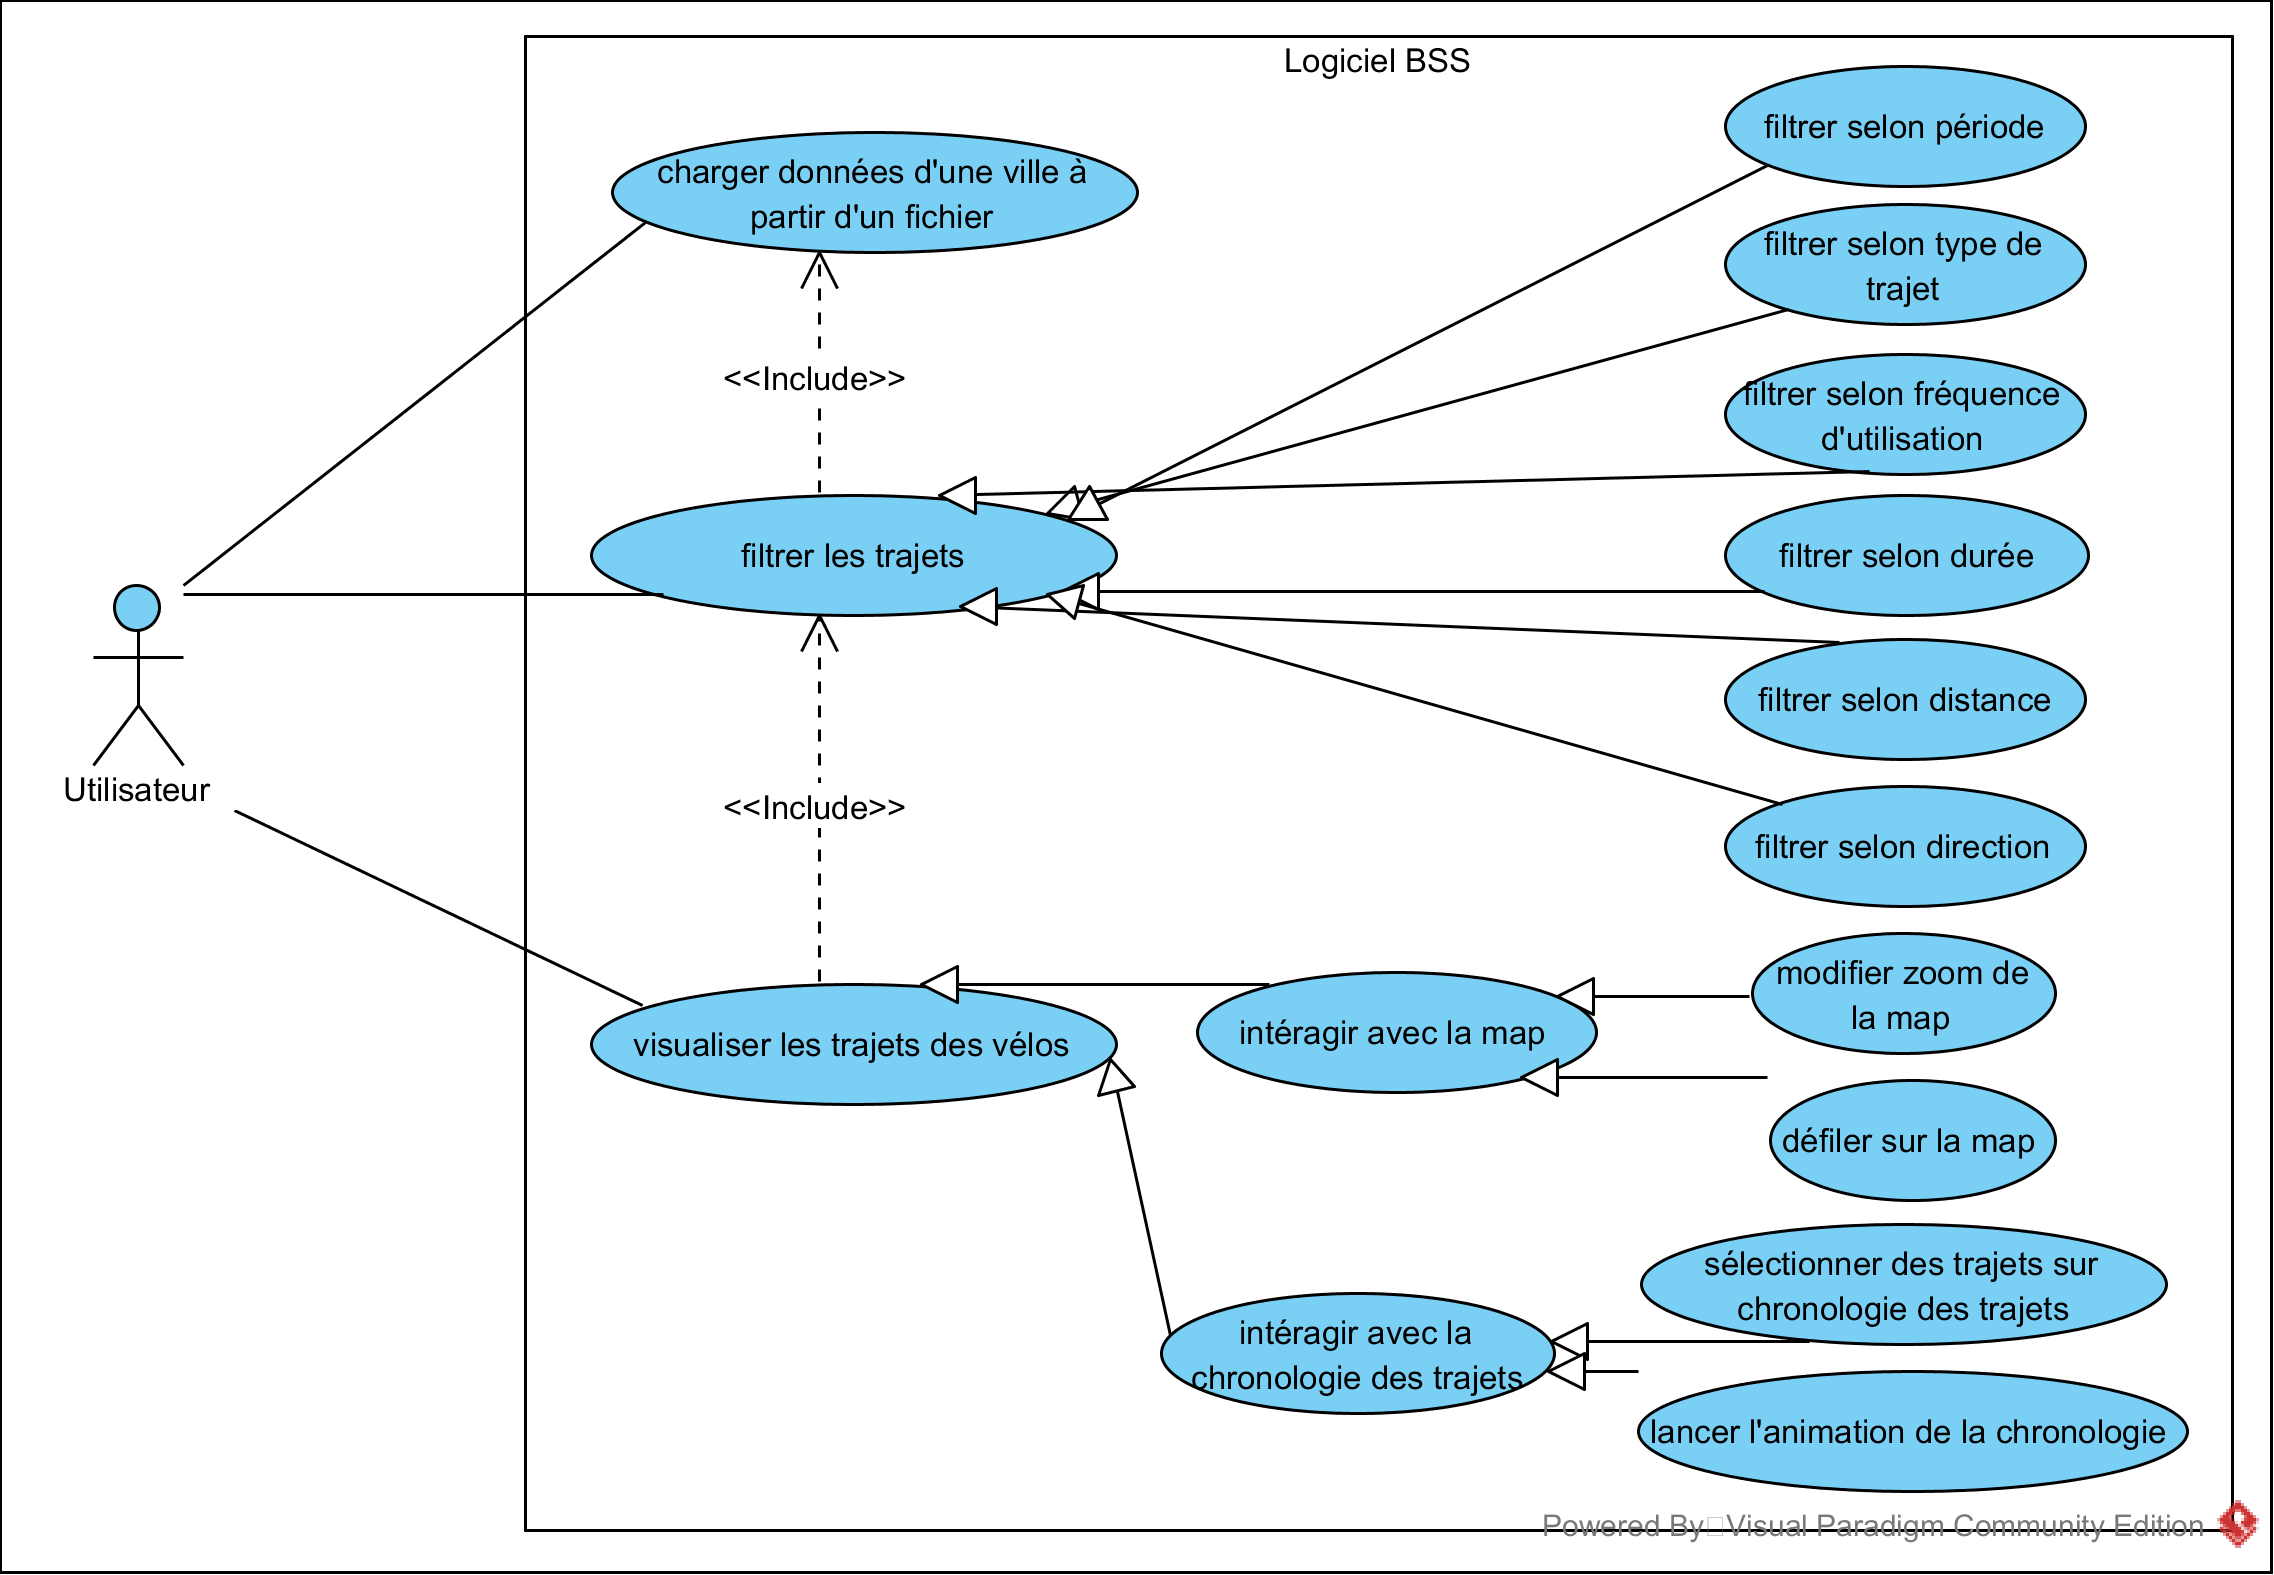
\includegraphics[scale=1]{Use_case_1.png}
		\caption{diagramme de cas d'utilisation du logiciel de Bike Sharing System (BSS)}
		\medskip
		L'utilisateur commence par charger les données des trajets pour une ville de son choix.\par

		Ensuite, il a la possibilité de filtrer les trajets qu'il souhaite visualiser selon plusieurs critères :\\
			-selon la période : un jour particulier, un jour de la semaine, le weekend, les jours ouvrés\\
			-selon le type de trajet : les départs, les arrivées, les trajets cycliques\\
			-selon la fréquence d'utilisation des vélos\\
			-selon la durée des trajets, leurs distances, leurs directions\\
		Lorsqu'un paramètre de filtrage est modifié, la chronologie des trajets est rafraîchie.\par

		Une fois que l'utlisateur a filtré les trajets selon ses besoins, il peut intéragir avec la map pour la faire défiler ou en modifier le niveau de zoom.\\
		Il peut aussi intéragir avec la chronologie des trajets en sélectionnant les trajets de stations particulières.\\
		Les trajets des stations selectionées sont affichés sur la map.\\
		Il peut enfin lancer l'animation de la chronologie en appuyant sur un bouton "play" : l'activité d'utilisation défile dans le temps.
		\end{figure}
		\newpage

		\subsection{Besoins fonctionnels}
			\subsubsection{Visualisation de la carte de la ville}
				\begin{itemize}
					\item fenêtre pour visualiser les trajets de manière géographique avec une map
					\item map d'une ville chargée avec OpenStreetMap
					\item la map affiche uniquement les stations de la ville lorsqu'il y a des stations sélectionnées dans la matrice de chronologie, elle n'affiche que celles-ci (ainsi que les trajets qui y sont associés)
					\item les trajets sont dessinés par des courbes avec un dégradé de deux couleurs
					\item les départs sont dessinés du cyan (station d'origine) vers le bleu (station de destination) dans le sens horaire
					\item les arrivées sont dessinées du rouge (station d'origine) vers le jaune (station de destination) dans le sens anti-horaire
					\item lorsque l'utilisateur passe sa souris sur une station de la map, la ligne associée à la station est surlignée en noir dans la matrice de chronologie des trajets
					\item lorsque l'utilisateur passe sa souris sur une station de la matrice de chronologie des trajets, la station est surlignée en noir sur la map
					\item L'utilisateur pourra faire un zoom avant ou un zoom arrière grâce à des boutons destinés à cet effet.
					\item Il pourra aussi se déplacer dans la carte, à gauche, à droite, en haut et en bas. Il réalisera cette action soit en appuyant sur des boutons, soit grâce à un système de glisser/déposer, afin de permettre une translation et se déplacer dans la carte.
				\end{itemize}

			\subsubsection{Matrice de la chronologie des trajets}
				\begin{itemize}
					\item axe horizontal : temps en heure (une colonne pour chaque heure)
					\item axe vertical : stations (une ligne pour chaque station)
					\item les stations sont représentées dans des cellules par des petites étoiles (les lignes étant les trajets, représentés avec leurs directions et leur longueur)
					\item arrivées en rouge
					\item départs en bleu
					\item trajets cycliques par des cercles transparents dont le rayon est proportionnel à la distance du trajet
					\item les stations pour lesquelles il n’y a plus de places disponibles (“full outage”) sont encadrées en rouge
					\item les stations pour lesquelles il n’y a plus de vélos libres (“empty outage”) sont encadrées en bleu
					\item possibilité de sélectionner les stations avec la souris, selon une intervalle horaire
					\item les stations sélectionnées dans cette fenêtre sont visibles sur la map, avec les trajets qui y sont associés
					\item possibilité de dérouler, sur 24 heures, l'activité des emprunts des vélos en lançant l'animation (en appuyant sur le bouton play)
				\end{itemize}

			\subsubsection{Interface de selection de filtres}
				\textbf{Possibilité de pouvoir filtrer dans le temps}\par
					\begin{itemize}
						\item un mois et son année : menu déroulant avec choix chargés à partir de fichiers données
						\item un jour précis : entrée du jour du mois (un entier compris 1 et 31) dans un champ de texte 
						\item jour de la semaine/jours ouvrés/weekend\\
					\end{itemize}

				\textbf{Possibilité de filtrer selon les propriétés des trajets}\par
					\begin{itemize}
						\item arrivées : si cochée, affiche (en rouge) les trajets arrivants, sur la map ainsi que dans la chronologie des trajets
						\item départs : si cochée, affiche (bleu) les trajets partant, sur la map ainsi que dans la chronologie des trajets
						\item trajets cycliques : si cochée, affiche (par un cercle gris transparent dont le rayon est proportionnel à la longueur du trajet) les trajets cycliques, dans la chronologie des trajets
						\item durées des trajets : si cochée, prend en compte la durée des trajets
						\item longueurs des trajets : si cochée, prend en compte la longueur des trajets (les longueurs des traits des trajets dans chaque cellule de la chronologie des trajets sont relatives au trajet le plus long), sinon, tous les  traits sont de même longueur
						\item interruptions/pannes : si cochée, encadre les stations, dans la chronologie des trajets, en rouge s'il n'y a plus de places de libres ("full outage"), en bleu s'il n'y a plus de vélos libres ("empty outage")\\
					\end{itemize}

				\textbf{Filtrer selon des valeurs entières comprises dans un intervalle borné par une valeur minimale et une valeur maximale}\par
					\begin{itemize}
						\item longueur (en mètres) : min = 0, max = 14000
						\item durée (en minutes) : min = 0; max = 120 
						\item direction (en degrés) : min = 0, max = 360
						\item flux d'origine-destination : min = 0, max = 1000
					\end{itemize}

		\subsection{Besoins non fonctionnels}
			\subsubsection{Interfaces}
				\begin{itemize}
					\item Le texte de l'interface graphique sera en anglais.
				\end{itemize}

			\subsubsection{Affichage des trajets}
				\begin{itemize}
					\item Les trajets seront affichés sur la carte par des courbes depuis le points de départ du trajet jusqu'au point d'arrivée.
					\item Les points de départs seront de couleur rouge et les points d'arrivées seront de couleur jaune.
				\end{itemize}

			% \subsubsection{Les filtres}
			% 	\begin{itemize}
			% 		\item 
			% 	\end{itemize}

			\subsubsection{Performances}
				\begin{itemize}
					\item Afin d'assurer la fiabilité du logiciel, des tests unitaires seront réalisés avec Banditcpp. 
					\item L'application doit s’exécuter rapidement sur une carte graphique Quadro K2000M :
					\begin{itemize}
						\item Lors de la lecture du fichier
						\item Lors de l'affichage des données
						\item Lors de l'application des divers filtres
						\item Lors du déplacement sur la carte
					\end{itemize}
				\end{itemize}

			\subsubsection{Dévelopement}
				\begin{itemize}
					\item Le code devra être très bien documenté, Doxygen, est un outil qui permet la génération de documentation. Un manuel latex sera généré.
					\item La dernière version de Qt sera utilisée, à l'heure actuelle, c'est la version 5.8 stable.
					\item Pour le rendu graphique, la version d'OpenGL doit être superieure à la version 3.2. Ainsi, aucune fonction obsoléte ne sera utilisée.
					\item Le code C++ sera compilable avec le compilateur g++ 5.9.
					\item L'application devra forcément tourner sur une carte NVIDIA.
				\end{itemize}
	\newpage

	\section{Les livrables}
		Le mercredi 5 avril, tout le code source bien commenté, ainsi qu'un fichier exécutable sera remis. Une documentation détaillée sur la manière d'utiliser le logiciel accompagnera le code source.
	\newpage

	\bibliography{bibliographie}

\end{document}
